\section{GIÁ TRỊ LƯỢNG GIÁC CỦA MỘT GÓC TỪ $0^\circ$ ĐẾN $180^\circ$}
\subsection{TÓM TẮT LÝ THUYẾT}

\subsubsection{Giá trị lượng giác của một góc}
\begin{itemize}
	\item [\iconMT] \indam{Định nghĩa:} Với mỗi góc $\alpha$ $(0^\circ\le \alpha \le 180^\circ )$, ta xác định duy nhất một điểm $M$ trên nửa đường tròn đơn vị sao cho $\widehat{xOM}=\alpha $. Giả sử điểm $M$ có tọa độ $M(x_0;y_0 )$, khi đó ta có định nghĩa:
	\begin{gachsoc}
	\immini{\begin{itemize}
			\item  sin của góc $\alpha $ là $y_0$, kí hiệu $\sin \alpha$. 
			\item  cosin của góc $\alpha $ là $x_0$, kí hiệu $\cos \alpha$.
			\item tang của góc $\alpha $ là $\dfrac{y_0}{x_0}\,\,(x_0\ne 0 )$ ,
			kí hiệu $\tan \alpha$. 
			\item cotang của góc $\alpha $ là $\dfrac{x_0}{y_0}\,\,(y_0\ne 0 )$, kí hiệu $\cot \alpha$.
		\end{itemize} 
	}{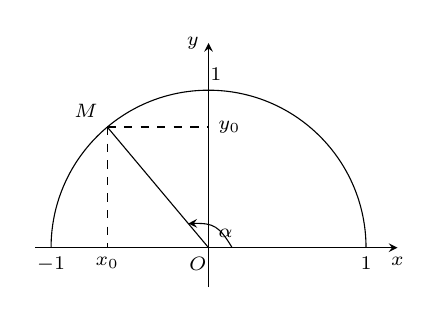
\begin{tikzpicture}[>=stealth,font=\scriptsize]
			\draw[->] (-2.2,0) -- (2.4,0) node[below]{$x$};
			\draw[->] (0,-.5) -- (0,2.6) node[left]{$y$};
			\draw (.1,0) node[below left]{$O$}
			(-2,0) node[below]{$-1$}
			(2,0) node[below]{$1$}
			(-0.1,2) node[above right]{$1$};
			\draw (2,0) arc (0:180:2cm);
			\path (130:2cm) coordinate (M);
			\draw[dashed] (M) node[above left]{$M$} -- (M|- 0,0) node[below]{$x_0$};
			\draw[dashed] (M) -- (M -|0,0) node[right]{$y_0$};
			\draw (0,0) -- (M);
			\draw[->] (0.3,0) to [bend right,looseness=1.3] (130:0.4cm) node[above right,midway]{$\alpha$};
	\end{tikzpicture}}
	\end{gachsoc}
\indamm{Từ định nghĩa trên, ta có:}
\begin{tcolorbox}[colframe=orange,colback=white,boxrule=0.2mm]
	\begin{listEX}[3]
		\item [\ding{172}] $\tan \alpha=
		\dfrac{\sin\alpha}{\cos\alpha}$
		\item [\ding{173}]  $\cot \alpha=
		\dfrac{\cos\alpha}{\sin\alpha}$
		\item [\ding{174}] $\tan \alpha=\dfrac{1}{\cot\alpha}$
	\end{listEX}
\end{tcolorbox}
	\item [\iconMT] \indam{Bảng giá trị lượng giác của góc đặc biệt:}
	\begin{center}
		\renewcommand{\arraystretch}{2}
		\begin{tabular}{|c|c|c|c|c|c|c|}
			\hline
		 & $0^\circ$ & $30^\circ$ & $45^\circ$ & $60^\circ$ & $90^\circ$ & $180^\circ$\\
			\hline
			$\sin \alpha$  & $0$ & $\dfrac{1}{2}$ & $\dfrac{\sqrt{2}}{2}$ & $\dfrac{\sqrt{3}}{2}$ & $1$ & $0$\\
			\hline
			$\cos \alpha$  & $1$ & $\dfrac{\sqrt{3}}{2}$ & $\dfrac{\sqrt{2}}{2}$ & $\dfrac{1}{2}$ & $0$ & $-1$\\
			\hline
			$\tan \alpha$ & $0$ & $\dfrac{1}{\sqrt{3}}$ & $1$ & $\sqrt{3}$ & $\big|\big|$ & $0$\\
			\hline
			$\cot \alpha$ & $\big|\big|$ & $\sqrt{3}$ & $1$ & $\dfrac{1}{\sqrt{3}}$ & $0$ & $\big|\big|$\\
			\hline
		\end{tabular}
	\end{center}
\end{itemize}
\subsubsection{Mối quan hệ giữa các giá trị lượng giác}
\begin{itemize}
	\item [\iconMT] \indam{Hai góc bù nhau:} Trên hình bên ta có dây cung $NM$ song song với trục $Ox$ và nếu $\widehat{xOM}=\alpha $ thì $\widehat{xON}=180^\circ-\alpha $. Ta có $y_{M}=y_{N}=y_0,$ $x_{M}=-x_{N}=x_0$. Do đó
	\begin{gachsoc}	
			\immini{
			\begin{listEX}[1]
			\item [\ding{172}] $\sin (180^\circ-\alpha )=\sin \alpha$
			\item [\ding{173}] $\cos (180^\circ-\alpha )=-\cos \alpha$
			\item [\ding{174}] $\tan (180^\circ-\alpha )=-\tan \alpha$
			\item [\ding{175}] $\cot (180^\circ-\alpha )=-\cot \alpha$
		\end{listEX}
	}{\begin{tikzpicture}[scale=1, font=\footnotesize,>=stealth,x=2cm,y=2cm]
			\def\x{0.715}
			\def\a{44}
			\pgfmathsetmacro{\y}{\x*tan(\a)}
			\draw[->] (-1.3,0)--(1.3,0) node [below]{$x$};
			\draw[->] (0,-0.2)--(0,1.3) node [left]{$y$};
			\node at (0,0) [below left]{$O$};
			\draw (1,0) arc (0:180:2cm);
			\fill (1,0) node[below]{$1$} circle(1pt);
			\fill (-1,0) node[below]{$-1$} circle(1pt);
			\fill (0,1) node[above left]{$1$} circle(1pt);
			\fill (\x,0) node[below]{$x_0$} circle(1pt);
			\fill (-\x,0) node[below]{$-x_0$} circle(1pt);
			\fill (\a:1) node[above right]{$M$} circle(1pt);
			\fill (180-\a:1) node[above left]{$N$} circle(1pt);
			\fill (0,\y) node[above right]{$y_0$} circle(1pt);
			\draw[dashed] (\x,0)|-(0,\y);
			\draw[dashed] (-\x,0)|-(0,\y);
			\draw (44:1)--(0,0)--(136:1);
			\draw (0.3,0) arc (0:\a:0.6cm);
			\node at (0,0)[shift={(25:0.2)}]{\tiny{$\alpha$}};
			\draw (0.2,0) coordinate (A) -- (0,0) coordinate (B) -- (136:0.6 cm) coordinate (C) pic [draw, double, angle radius = 9mm] {angle = A--B--C}; 
			\draw (0.25,0.55)node{\tiny{$180^\circ-\alpha$}};
	\end{tikzpicture}}
		\end{gachsoc}
	\item [\iconMT] \indam{Hai góc phụ nhau:} Hình vẽ bên, hai điểm $M$ và $N$ ứng với hai góc phụ nhau $\alpha$ và $90^\circ-\alpha$ ($\widehat{xOM}=\alpha$, $\widehat{xON}=90^\circ-\alpha$ )
	\begin{gachsoc}
		\immini{	\begin{itemize}
				\item [$\bullet$] $\cos \left( 90^\circ-\alpha  \right) = \sin \alpha$
				\item [$\bullet$] $\sin \left(90^\circ-\alpha  \right) = \cos \alpha$
				\item [$\bullet$] $\tan \left(90^\circ-\alpha  \right) = \cot \alpha$
				\item [$\bullet$] $\cot \left( 90^\circ-\alpha  \right) = \tan \alpha$
			\end{itemize}
		}{
			\begin{tikzpicture}[scale=1, font=\footnotesize,>=stealth,x=2cm,y=2cm]
				\def\x{0.866}
				\def\a{30}
				\pgfmathsetmacro{\y}{\x*tan(\a)}
				\draw[->] (-1.3,0)--(1.3,0) node [below]{$x$};
				\draw[->] (0,-0.2)--(0,1.3) node [left]{$y$};
				\node at (0,0) [below left]{$O$};
				\draw (1,0) arc (0:180:2cm);
				\fill (1,0) node[below]{$1$} circle(1pt);
				\fill (-1,0) node[below]{$-1$} circle(1pt);
				\fill (0,1) node[above left]{$1$} circle(1pt);
				\fill (\x,0) node[below]{$x_0$} circle(1pt);
				\fill (\a:1) node[above right]{$M$} circle(1pt);
				\fill (90-\a:1) node[above right]{$N$} circle(1pt);
				\fill (0,\y) node[above left]{$y_0$} circle(1pt);
				\draw[dashed] (\x,0)|-(0,\y);
				\draw[dashed] (\y,0)|-(0,\x);
				\draw (\a:1)--(0,0)--(90-\a:1);
				\draw (0.3,0) arc (0:\a:0.6cm);
				\node at (0,0)[shift={(15:0.25)}]{\tiny{$\alpha$}};
				\draw (0.2,0) coordinate (A) -- (0,0) coordinate (B) -- (90-\a:0.6 cm) coordinate (C) pic [draw, double, angle radius = 9mm] {angle = A--B--C}; 
				\draw (0.55,0.3)node{\tiny{$90^\circ-\alpha$}};
		\end{tikzpicture}}
	\end{gachsoc}
\end{itemize}
